\begin{figure}[t]
    \centering
    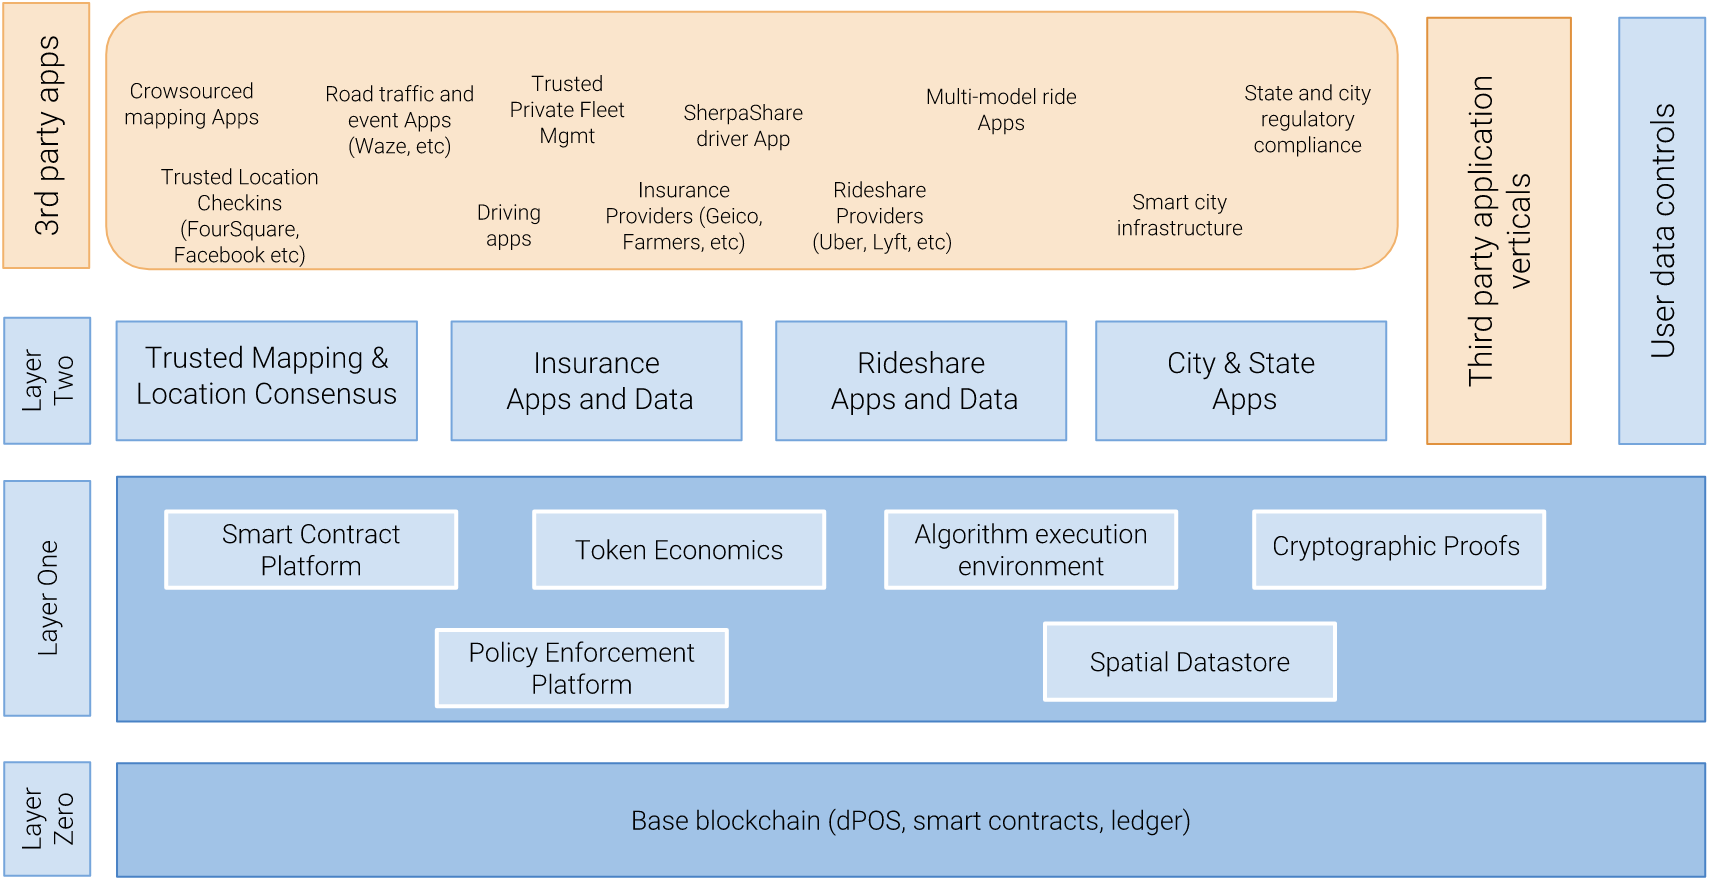
\includegraphics[width=1.00\textwidth]{lat-arch-2.png}
  \caption{Architecture of the Latitude Blockchain and associated platform ecosystem.}
    \label{fig:lat-arch}
\end{figure}

\section{The Latitude Platform}\label{sec:design}

In this Section, we present a high-level design of the Latitude platform.  We start with an overview of the key design
principles that will guide the rest of the design for Latitude. Its important to note here that for implementation
purposes, it might be possible to use an existing core blockchain for the underlying functionalities and build Latitude
as a layer on top.

The purpose of the Latitude platform is to become the best blockchain-based ecosystem in the world for decentralized
applications for the Transportation Industry. Specifically, this boils down to constructs in the blockchain that can
handle spatial, mapping, traffic, driving data including data relating to other modalities of transport (bike sharing,
walking, even air routes later on). Figure \ref{fig:lat-arch} presents the architecture of the Latitude blockchain in
terms of the core technological innovations that will be built into it.

\subsection{Architecture overview}

The overall architecture of the Latitude Blockchain consists of a base blockchain and a protocol implementation (Dapp
SDK and smart contract APIs) for each application vertical. This choice of an architecture gives the maximum flexibility
for each application vertical to use its own protocol mechanisms for token incentives while allowing for summaries or
Merklized proofs of transactions to be commited to the base chain. In the first (few) version of Latitude, the base
chain might be an existing blockchain such as Ethereum, EOS, Zilliqa or Neo. Eventually Latitude might move to a
specialized design of a blockchain that works well for Transportation data and dapps. The specific mechanisms for each
business vertical shall be discussed in Section \ref{sec:apps}.

\begin{itemize}
    \item Overall architecture.
    \item Side chains. Main chain.
    \item chains interact mechanism.
    \item Cross-chain transactions are commitment protocol.

\end{itemize}

Each application vertical utilizes atleast one side-chain. Depending on the application, it might be necessary for
multiple side-chains to exist within a vertical, in which case we shall use composable side-chains similar to Plasma.
This allows for a hierarchical side-chain structure if needed with eventual commitment to the mainchain.

Implementation Note: For the alpha version of Latitude, it might be possible to use an existing chain with high
transaction velocity and low cost, such as EOS, Neo, Zilliqa or Harmony as a drop-in replacement for the base chain
functionality. In the long term, it might be beneficial to have our own base-chain with built in smart contract
functions for transportation applications. This will also work better with Latitude's own token economics.

\noindent
{\em Base Blockchain layer:}

The Latitude platform uses a base blockchain layer for Layer-0 operations as shown in Figure \ref{fig:lat-arch}. The
base layer can be an existing blockchain so that the Latitude essentially provides middleware for layer 2 and 3
operations. This design shall be sufficient for the first few versions of Latitude. Long term we shall migrate to our
own base blockchain to help scale operations that work better for the Latitude dapps.

Delegated Proof of Stake (DPOS) is a fast, efficient and decentralized consensus model available today. DPOS
leverages the power of stakeholder approval voting to resolve consensus issues in a fair and democratic way. All network
parameters, from fee schedules to block intervals and transaction sizes, can be tuned via elected delegates.
Deterministic selection of block producers shows that transactions can be confirmed in an average of less than a second
\cite{eos_producers}. This speed is important for scaling the Latitude chain.

Latitude's Delegated proof of stake system uses a set of "delegates" for voting on a block producer. The delegates are
"promoted" based on time-based trust or stake (or a combination of these). This design is similar to the Cosmos
blockchain and differs from other dPOS system such as EOS. The exact number of delegates can be a tunable parameter that
can be changed by the governing council of nodes. This version of takes the best of both cooperative and competitive
consensus algorithms.  The competitive part is larger stakeholders having an influence on their delegate of choice. In
Latitude, it is also possible to gain a larger stake by accruing what we call "trust" through honest operation over a
period of time. The delegates that have the most votes will take their turn to produce a block cooperatively in a
sequence. A $2/3$ majority of consensus among the delegates over the {\em last minted block} is needed to achieve
consensus and mint a new block onto the chain. Further discussion on Governance and other paremeters of a custom
Blockchain design are discussed in Appendix \ref{app:latchain}.

\subsection{Spatial datastore}
One of the central aspects of the Latitude blockchain is a geo-spatial datastore that fundamentally understands various
datatypes that are specific to transportation data. This datastore can use existing GIS databases that allow
de-centralized storage and access. The types of data include (i) geographic data such as location (latitude, longitude),
(ii) mapping data such as roads, terrain, addresses, etc, (iii) sensor data such as driving data, driver score, miles
driven, route information, etc, (iv) multi-modal transport data such as biking, walking and other means of transport.
Each of these data types have very special characteristics which the underlying datastore can be optimized for and allow
for programming using what we call the {\em Latitude Smart Contract} framework. 

The datastore would include spatial, quad-tree or an R-tree based indexes for efficient querying and other operations that
most Geographic Information Systems (GIS) would support in a centralized manner today. It would also include functions
to compute heatmaps, driving maps and statistics such as Traffic predictions including real-time analytics. Depending on
how Latitude evolves, the datastore can include additional functionalities to support the data sharing among autonomous
vehicles since they use most of the similar datatypes mentioned above. The datastore would support circular, rectangular
and other range queries, K-nearest neighbor searches, route optimization algorithms, etc. Figure
\ref{fig:geo_spatial_query} shows some of the queries that such a datastore can support.

%Datastore
% - Optimized for Geographic, Geo-spatial data.
% - Location, Mapping data and computation.
% - Ability to Store, index, query and build smart contracts optimized for such data.
% - Support for various spatial indexes.
% - Location heatmaps.
% - Indexing road and driving data.
% - Primitives for storing driving data for autonomous vehicles

\subsection{Trust Ledger}
\label{sec:trust}

One of the core concepts in Latitude is the presence of a decentralized trust and reputation managment system. Trust and
reputation systems have been widely used in e-Commerce applications. They are well understood in terms of attacks and
game theoretic models \cite{rahimi_2017, rahimi_2012}. Latitude uses trust as a way to reward participants who have been
{\em consistently} honest over a period of time. Trust is also central in creating proofs on Latitude as discussed in
Section \ref{sec:crypto}.

The Trust ledger is a decentralized ledger accessible to everyone in the system. It consists of a trust model where each
participant's trust is stored and updated through specific operations. The following salient points explain the design
of the trust model in Latitude:

\begin{itemize}
    \item Trust is gained via honest operation: Each honest operation by a participant helps increase its trust value.
        The decision of whether an operation is completed honestly happens through consensus on a smart contract and
        depends on the specifics of an operation. For example, successful proofs of location or being a participant in
        proving other's location helps increase trust. As another example, reliable operation in contributing resources
        such as disk, network etc also helps increase trust.
    \item Trust is different from stake: Stake is purely a measure of the amount of LAT token held by an entity. While
        it gives economic incentives for entities to operate honest, it does not capture long-term honest operation
        behavior that Trust and Reputation system can do \cite{dong_2010}.
    \item Trust depreciation: Trust can depreciate either through dis-honest or unreliable operation. This decision is
        also arrived via consensus on an operation-specific smart contract. For example, if a participant contributes
        ride-sharing data which is shown to be flawed (possibly using a trusted party such as an Uber-API call),
        the trust level for this participant gets drained. Trust can also {\em decay} over time if nodes do not
        participate in network operations. Thus, there is a freshness dimension to the trust value in Latitude.
\end{itemize}

\noindent
{\em Half-life based exponential Trust decay:}
Trust in Latitude can decay over time in a way that is similar to how radioactive elements decay
using an half-life based formula shown below. This is to ensure that the trust values reflect freshness in operation.
The half-life value is a controllable parameter which indicates the duration after which the trust gets halved.
\begin{equation*}
    \label{eq_trust_decay}
    N(t) = N_0 \bigg(\frac{1}{2}\bigg)^\frac{t}{t_{1/2}}
\end{equation*}
where 
\begin{itemize}
    \item $N(t)$: The amount of trust at time $t$.
    \item $N_0$: The amount of initial trust before decay.
    \item $t_{1/2}$: Half-life of the trust decay model.
\end{itemize}

The amount of trust is used in Latitude to create proofs for various observations such as Location, Mapping, Traffic
etc. A combination of trust and stake are used in the DPOS and Governance operations.

\subsection{Cryptography layer} \label{sec:crypto} Latitude makes use of state-of-the-art cryptographic protocols to
provide various proofs, access control, confidentiality and other properties that are important in a decentralized
system.

such as AES encryption, secure hash functions, PKI certificates, multi-party key distribution protocols, proxy key
re-encryption schemes, Elliptic-curve based Digital Signatures \cite{ecdsa}. They help provide strong security, privacy,
access control, confidentiality and anonymity guarantees. Anonymity guarantees are an important part of data-sharing
smart contracts and privacy policies such as GDPR \cite{gdpr} especially for geo-spatial data such as location and maps.
Latitude provides anonymity guarantees using cryptographic set-preserving computations as derived from research in
\cite{kissner_set}. These can be suitably modified to allow for location-based anonymity which require stronger
guarantees when compared to set-based anonymity methods \cite{divanis_kanon,xu_loc_anon}.

Latitude also uses Merkle trees for cryptographic proof of audit, existence of data and verifiable computations
\cite{becker2008}. These proofs can be shared as certificates among participants or be used in the Latitude smart
contract system discussed later. They allow for verification of data existence or data-sharing contracts. They also
allow for the maintenance of a cryptographic log of all operations that happen on the network. These techniques are
similar to the ones used by some of the other blockchains today \cite{buterin_merkle}.

\subsubsection{Integrity and Access Control}

Latitude uses standard and well understood cryptographic protocols to provide robust access control and maintain basic
integrity of transactions. Data integrity is maintained using digital signatures. Every transaction is signed by one or more of the participants
certificates. The blockchain ledgers are protected using a Merkle hash \cite{becker2008} as discussed in the previous
section. A Merkle proof is used as a proof of transaction for cross-chain communication.

Access control for data that is not public or open, can be managed using multi-party key communication protocol (MPC)
\cite{enigma, nucypher, mpc_survey}. MPC protocols work over a set of $N$ trusted participants or a consortium set. They
can be designed to allow a minimum of $m<N$ participants to reach a consensus (using a off-chain protocol) in order to
compute the key that would grant access. Using these primitives, it becomes possible to have granular access control,
such as different amount of consensus for read, for writes and other semantic actions. Latitude shall make these
mechanisms available to the app developer through platform APIs. As always, since this is an open system, it is possible
for developers to build their own access control methods if they so wish.

%Cryptographic primitives for:
% - Security and privacy of data.
% - Anonymity guarantees using cryptographic set operations.
% - Enforcement of privacy when sharing data.
% - Sharing of “computation” instead of data when possible.
% - For eg: Sharing of DriverScore using a vetted algorithm.
% - Sharing proximity to a landmark instead of lat/lng.
% - Ability to find bad actors.
% - Detect privacy, anonymity and security violations.
%
%Cryptographic proofs for applications:
% - Proof of Location. 
% - Proof of ride. 
% - Proof of mapping 
%      (road/landmark exists or does not exist).
% - Proof of driver score 
% - Open, trusted, understood driver score computation algorithms.
% - Cryptographic proofs can be shared among entities, safely, securely.

In addition to these standard primitives, Latitude provides a host of other proofs that are tailor made
for geo-spatial, mapping, location and sensor data. These proofs can be used by applications, users and
other participants in the network. The network can be extended to create new forms of proofs as the application needs
grow. Below, we present the core set of cryptographic proofs that are unique to the Latitude blockchain:

\begin{figure}[t]
    \centering
    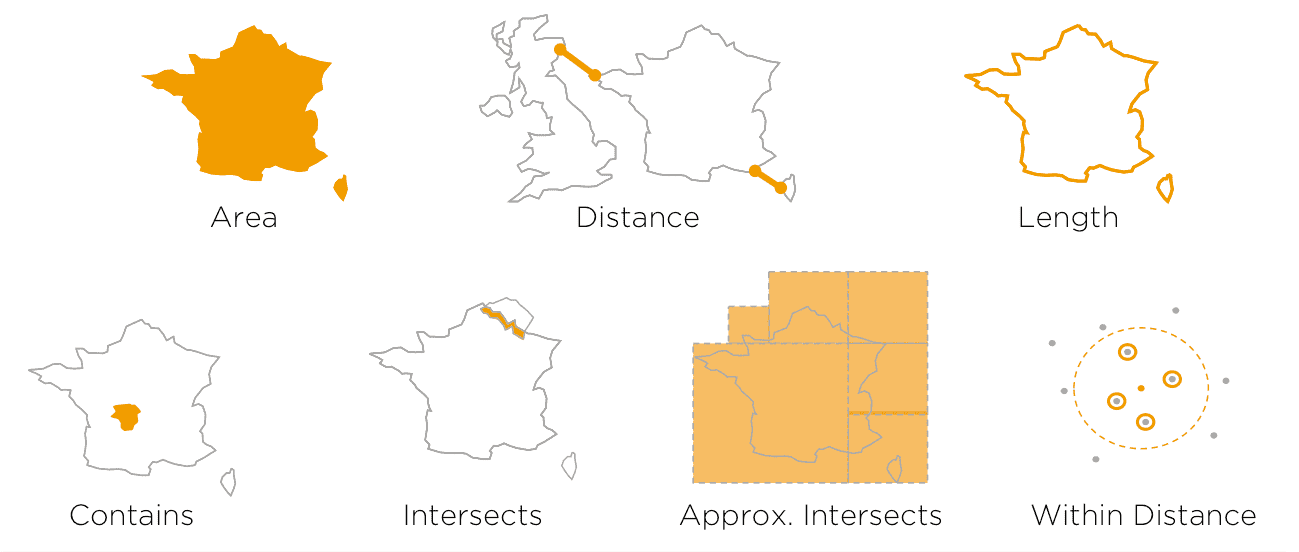
\includegraphics[width=0.70\textwidth]{geospatial_query.png}
  \caption{Examples of Geo-spatial queries that a spatial data-structure can support on the Latitude blockchain.}
    \label{fig:geo_spatial_query}
\end{figure}

\subsubsection{Proof of Real-world Observation}

A real-world observation could be a location computation, a ride from point A to B, a traffic observation or a landmark
at a given location. The core concept behind these observations is the flow of trust. The concepts presented in this
Section and the subsequent Sections replace and solve the offline Oracle problem that blockchains face today. These
mechanisms provide a practical method of creating a trust source of observation without requiring a perfect off-chain
Oracle \cite{concurrence}.

Any observation in the real world, be it a location or a landmark sighting is only as good as the trust placed in the
method and apparatus used to compute it. For example, if a GPS receiver returns a location, the amount of trust in that
location result is proportional to the amount of trust in the receiver construction and the satellite system being used
(such as Navstar, GNSS or others). Latitude uses this concept of trust as an internal metric to compute a proof of a
real-world observation.  Here we present the common algorithm used to compute these proofs which can be shared across
the Latitude platform.

\newcommand\NF{\mathit{Nf}}
\newcommand\TM{\mathit{Tm}}
\noindent
{\bf Definitions:}
\begin{itemize}
    \item Levels of trust $t_i, i \in \{0..M\}$, where $M$ is the max level of trust in the system. Trust level $t_{i+1} >
        t_i$.
    \item $t_0$ is the base level of trust assigned to any third party untrusted source of data.

    \item Each data source (such an an app installation, or a third-party source) is indentified using a certificate's
        public key. If this is a fully untrusted source that belongs to a third party, they start at the lowest level of
        trust $t_0$.

    \item $t_1$ is the trust assigned to a second party integration with Latitude's SDKs where the SDKs directly compute the
        observation and report it to the system using second-party APIs. Examples include Apps in the trusted App stores
        that integrate with Latitude.
    \item $t_2$ is the trust assigned to a first-pary integration, such as a Latitude mobile app, or a first-party app
        from trusted partners such as SherpaShare.
    \item $tmin_{pf}$ is the minimum trust needed for a specific proof or obervation. Each proof type might have a
        different requirment for this parameter. The computed proof also carries this parameters as an indication of
        consensus or trust.
    \item Trust map, $\TM(e)$ gives the amount of trust recorded in the ledger for the entity $e$. The entity could be an
        organization, an individual or a user (as identified by an app installation, for example).
    \item $N_{min}$ is the minimum number of entities that need to participate in the creation of this proof. This can
        be a function of the proof being created.
    \item The entity requesting the proof, submits a request $R(e, t_b, V, \TM(e))$, where $R$ represents the proof
        request. The request includes credentials for entity $e$, the base trust level in the request $t_b$, the
        evidence of real-world observation (such as radio signal strength) $V$ and the existing entry in the trust
        legder $\TM(e)$.
    \item Concurrence Weight: Each witness that concurs with an observation provides a {\em concurrence weight} which is
        the probability that they think the event happened. This is a value between 0 and 1. Denoted as $W_c(w, e, V)$,
        where the parameters are witness or observer $w$, entity $e$ and evidence $V$.
    \item Location specific trust normalization factor $\gamma_L$. $\gamma$ for a location $L$ is a location specific
        normalization factor which represents the average trust consensus in a specific location. For example, certain
        areas might have a higher concentration or honest or dishonest nodes. Or certain methods of location
        determination might have a bias that needs to be factored in.
\end{itemize}

Each proof is implemented as a special smart contract supported by the Latitude platform. The smart contract that
computed these proofs would provide a signed blob of data that certifies a certain observation as determined by the
respective proof.

\noindent
{\bf Algorithm for Proof of an observation $X$}:
\begin{enumerate}
    \item Suppose $e$ is the entity that initiates a request for proof of an obervation $X$ made by $e$.
    \item The proof system finds a subset (possibly randomly sampled) of participants $S$ who are able
        to {\it concur} with the obervation $X$. Each participant, $p_i \in S$, assigns a {\em concurrence} weight
        $W(p_i, X) \in [0,1]$ depending on how well they concur with the observation.
    \item Normalization factor $\NF(p_i, X)$: This is a multiplier, usually greater than 1, that signifies the
        amplification in trust as a funciton of how the observation was concurred upon. 
    \item Each observer $p_i \in S$, provides a normalization factor $\NF(p_i, X)$ and a concurrence weight $W(p_i, X)$
        to the proof.
    \item The proof computes the total trust in the observation $X$ as $T_{pf}(X, e, S)$, given by Equation
        \ref{eq_trust_compute}.
    \item Trust normalization: The total trust in $T_{pf}(X, e, S)$ gets normalized by $\gamma_L$ where $L$ is a coarse
        grained (city-level) location being considered. At bootstrap, a normalization factor of $1.0$ can be used.
\end{enumerate}

\noindent
Trust computation for a proof of observation X:
\begin{equation*}
    \label{eq_trust_compute}
    T_{pf}(X, e, S) = \sum_{i\in S} T(p_i) * \NF(p_i, X) * W(p_i, X)
    T_{pf}(X, e, S) = \gamma_L * T_{pf}(X, e, S)
\end{equation*}

where $T_{pf}(X, e, S)$ is the trust for the proof of observation $X$ proposed by entity $e$ and observed by
participants $S$. A proof is considered valid if $T_{pf}(X, e, S) > tmin_{pf}(X)$, that is, the accumulated trust is
above the minimum required for the type of observation $X$.

\noindent
Trust updates: Once a proof gets computed, the entity that initiated the observation gets its trust updated using an
EWMA formula. Assuming entity $e$ gets its trust updated for a proof $p_e$:
\begin{equation*}
    T(e)_{p_e} = (1 - \alpha) * T(e) + \alpha * T(p_e) / |S|
\end{equation*}

The goal of the above formula is multi-fold:
\begin{enumerate}
    \item To increase the average trust in an entity $e$ as a function of successful proofs. The larger the number of
        successful proofs, higher is the average trust in the entity.
    \item Similarly, the goal is also to reduce trust in case, with adequate participants, the system was unable to
        verify the claim. In fact, a larger draining of trust shall be instrumented if the system finds the claim to be
        demonstrably false.
    \item Malicious behavior: If an observer or the entity consistently disagrees with others in the proof system,
        over time their trust level will get degraded using a gradient method used in other reputation systems
        \cite{sen2010}.
    \item Rewarding honest behavior: Over time as observers and entities produce results with consistency, their
        historicla reputation gets better and recorded in the trust ledger.
\end{enumerate}

\subsubsection{Proof of Location:}

This is perhaps the most easily motivated functionality that the Latitude blockchain can provide. Proof of location is a
proof of real-world observation that proves that a given user, entity or participant is/was physically present at a given
location at a specific time. The location could also be relative to another participant or landmark.

Latitude shall provide the mobile, browser and sensor SDKs that can directly tie into the datastore to provide consensus
based proofs. These proofs can unlock applications such as access to facilities or help increase trust in crowd-sourced
mapping, traffic and incident reports.

The proof of location uses the above framework for a real-world observations with the following specification:
\begin{itemize}
    \item Entity $e$ computes a location on a mobile device. This could be an Android/iOS phone or a tablet/laptop.
        Depending on how the entity uses Latitude's SDKs, the location computation starts with a base trust level of
        $t_0$, $t_1$ or $t_2$.
    \item As a part of the location proof request $R(e, t_b, \TM(e), V)$, the entity can submit any evidence $V$ that would help
        prove the location. For example, on Android, this can include wifi-radio signals, cell tower signals, GPS
        satellite location and timing signals, Bluetooth-LE scans, and other signals that can help prove the location.
    \item Either the entity or the platform can find other participants for concurrence.
    \item Concurrence: A participant can concur by confirming the observations included in the evidence $V$. This can
        include, for example, a degree of concurrence or other factors that quantify how well they concur. The degree of
        concurrence can be a function of the radio signal properties \cite{mishra_secure, Mathur_2011}. This is used to
        compute the concurrence metric $W_c(w, e, v)$.
    \item Depending on the trust level of the observer, or for other considerations, the normalization factor can be
        used to boost or marginalize the contribution from a witness or observer $w$, denoted by $\NF(w, e, V)$.
    \item The witnesses or observers independently submit their recordings to the smart contract system, which either
        generates a valid proof or declines the request. At the end of each such operation, the new trust levels for
        various entities are computed.
    \item Historical Location: A past location proof from the same entity can be used as a "virtual observation" if the
        location computation is in the recent past. This combined with reasonable laws of Physics or motion can provide
        a small amount of trust for the current proof. For instance, if the entity was spotted at a grocery store about
        5 minutes in the past, then any new location update that is within a few miles of the grocery store could be trusted.
    \item Using the proof equation \ref{eq_trust_compute}, a trust level and proof is computed.
\end{itemize}

The location proof and the corresponding data including trust parameters are recorded in a web-friendly format (such as
JSON/XML) on a ledger specifically used for such proofs. The ledger entry can be used as a URL to refer to this proof
for other applications that can be built on top of it.

\noindent
{\em Other proof of location chains:}
The framework provided by Latitude is general enough to capture different implementations. For instance, \cite{foam}
uses a trusted set of radio beacons or "anchors" to provide location signals. These essentially become highly trusted
observers or participants in our framework as they are essentially first-party observers (with a large amount of
base-level trust). As another example, Platin is a blockchain designed specifically for a proof of location. Their use
of sensors and increase in trust over time falls in line with the general concept of proof of obervation (possibly with
different trust constants).

\subsubsection{Proof of Ride}

Provides a proof that a particular user has taken a ride from point A to point B using a
certain type of transport. This proof can be used across multi-modal ride platforms such as bike or car rides.  This can
be extended to include bus trips, flights, train rides and so on. The proof of ride credential will be available via the
Latitude mobile SDK on various platforms. Using the mobile SDK to construct these proofs also adds to the amount of
trust on the nature and parameters of the ride.  

The proof of ride is computed using a time series of location updates. A Hidden Markov Model or other methods
\cite{wu2011} can be used as "algorithmic observers or verifiers" of a location trace. The location trace can be
supplanted with sensor data collected using a direct integration of the Latitude SDK. The sensor data should be in full
correlation with the location trace and would consistute the evidence set $V$ for this proof.

The proof of ride algorithm is the following:
\begin{itemize}
    \item Entity submits an evidence $V$ which includes a series of locations, or proof of locations and sensor data.
    \item Platform can compute the trust as a function of trust inherent in included locatin proofs. Also, in certain
        cases, it might be possible to have other observers to correlate the ride (such as passengers or drivers in a
        rideshare scenario).
    \item Algorithmic observers such as physical properties of the ride can also be used to add trust to the system.
    \item Trusted observers: A small set of trusted observers such as API-based verification from Rideshare systems like
        Uber, Lyft and others can also be used as verifiers or concurrence providers to augment the proof.
    \item Depending on how well the observations correlate, the computed final trust is used to compute a proof of ride.
\end{itemize}

Proof of ride becomes a blob of signed data which gets recorded on the ledger.

\subsubsection{Proof of Landmark}

This proves the existence of a particular landmark such as a monument, a building, a sign post at a given lat/lng. This
can also be used to prove the existence of a particular road or the lack of. These proofs can be constructed using the
proof of location combined with consensus among users.  This proof can become the backbone for verified mapping and
landmark data-based applications.

The proof of landmark works as follows:

\begin{itemize}
    \item Multiple observers send evidence for a landmark. Evidence can include GPS-tagged photos or other sensor data
        (including 3D data of the area) using Latitude-integrated apps.
    \item Any observer or entity can request the proof. It might also
        be possible for the system to create a proof automatically based on sufficient collection of evidence.
    \item Based on the strength of individual observations, a smart contract can create such proofs.
\end{itemize}

The proof of landmark can be used for mapping and other applications in the Geo-spatial location and mapping industry.
These proofs can be stored on the ledger and in a spatial database which can make for efficient querying.

\subsubsection{Proof of DriverScore}

This proof can be computed on the blockchain over the data aggregated on the
datastore. The algorithm itself shall be made available to the nodes either as an executable docker image or an
open-source version. This allows different nodes to run the computation and create a certificate of driver score which
can then be attributed to the driver. This open framework can also allow different driver score algorithms to co-exist
in the system creating a community where better driver score algorithms can be agreed upon and used as the industry
standard.

A proof of DriverScore is computed as follows:
\begin{itemize}
    \item Driver score computation depends on the availability of open, trusted and benchmarked algorithms.
    \item The sensor data can be made available on a decentralized database or can run locally on the phone via
        integration with the Latitude SDK.
    \item The observers include location time series data that pass through HMM models for validation. For example,
        location and sensor data should make physical sense. Also they should be consistent with data from other
        drivers in the area in temporal proximity. Other validation includes co-riders in a ridesharing scenario. 
    \item Since this proof is very specific to each individual driver, it might take time for the system to be able to
        create enough trust in a single driver data report.
\end{itemize}

\subsubsection{Proof of Traffic}

Similar to the driver score, traffic is also an algorithm that looks at the statistics
of location and speed data on roads. The proof is similarly computed through consensus and recorded as a certificate on
the blockchain. The proof could be about real-time traffic or historic traffic patterns which can be shared with smart
city applications, the Census Bureau or other regulatory bodies.

Proof of traffic is computed as follows:

\begin{itemize}
    \item The traffic evidence consists of a location series including sensor data that can compute velocity,
        acceleration and other parameters. Usually a GPS location also includes a velocity vector.
    \item Proof of traffic can be computed by the system automatically upon gathering sufficient evidence from
        potentially unrelated observers or participants.
    \item Algorithmic verifiers will play a central role here as they are able to validate the traffic using time series
        location data, velocity vectors and correlation from multiple observers.
    \item Incident data which includes traffic incidents, constructions and other such events also can be part of this
        proof system and help augment the trusted in this proof.
    \item This is similar to a centralized traffic system such as one provided by Waze (or Google maps), except it is
        open, fully decentralized with the data available for any interested party to access.
\end{itemize}

\subsubsection{Proof of Route}

Similar to the functionality in the popular Waze app, this is about whether there exists
a certain route (or a better route) from point A to point B. More the consensus, higher the trust. For example, if a
user actually takes the route from A to B and provides a proof of ride, that helps create the proof of its existence.
This is useful for trusted and verifiable mapping / routing applications.

Proof of Route is computed as follows:

\begin{itemize}
    \item Just like a proof of ride, a proof of route consists of multiple location points in a time series.
    \item An algorithmic verifier, such as a HMM model could add to the validity of the route.
    \item Other observers could include participants who have also taken the same route at a recent times. These need
        not be ridesharing passengers.
    \item The Latitude platform, or an entity could propose a proof which can be executed upon sufficiently collected
        trusted evidence.
\end{itemize}

Proof of route can solve problems in mapping where the locals have the most up-to-date information on the routes, but
there is also an issue of trust. Major map providers such as Navstar, Google and others have way to crowdsource such
information with a reputation system in place to tackle malicious intent. Latitude's proof of route can solve this
problem to help provide reliable data for mapping applications.

\subsection{Latitude Smart Contract system}

\begin{figure}[t]
    \centering
    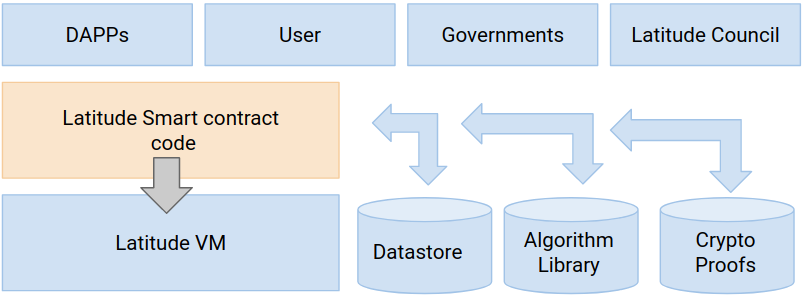
\includegraphics[width=0.60\textwidth]{lat_sc.png}
  \caption{Architecture of the Latitude Smart Contract framework.}
    \label{fig:lat-sc}
\end{figure}

Smart contracts are self-executing nuggets of code which specify the terms of the agreement between various participants
on the blockchain. For the Latitude blockchain, the participants can be a user, a regulatory body, an application
written by an insurance company or the city. The contract is directly written into lines of code in a certain smart
contract language. Popular smart contract frameworks today include ones used by Ethereum which runs on the Ethereum Virtual Machine (EVM),
the Neo which runs on the NeoVM and the EOS blockchain which runs on the WASM (WebAssembly VM).

The smart contract code and the agreements contained therein exist across the distributed, decentralized Latitude
blockchain network.  Because of this, Smart contracts permit trusted transactions and agreements to be carried out among
disparate, anonymous parties without the need for a central authority, legal system, or external enforcement mechanism.
They render transactions traceable, transparent, and irreversible as the state is always available on the Latitude
blockchain.

Figure \ref{fig:lat-sc} shows the high-level architecture of the Latitude Smart contract system. Latitude uses a
WebAssembly (wasm or eWasm) based compiler for a smart contract written in Go or C++. 

-- Overview of the webassembly architecture.

WebAssembly (or wasm) is a binary instruction format for a stack-based virtual machine. It includes a complier that is
portable and has a compilation target for high-level languages such as C++ and Go. The Latitude smart contract system
shall support both C++ and Go languages. The choice of wasm was to make the execution of the smart contract efficient
and thus have high throughput. Also, popular networks such as Ethereum are planning to move to eWasm as part of the
Ethereum Virtuam Machine (EVM) 2.0. This which will help create a common developer pool (and other aspects such as
tooling, educational material, etc) in the community. Wasm's execution happens in a safe and sandboxed
environment which can be beneficial in an adversarial and open network. It might also be possible to secure the Wasm
execution using Trusted Execution Environments (TEEs) in the near future.

The reason for chosing WebAssembly over the popular Solidity (or Vyper) used by the Ethereum Virtual Machine (EVM 1.0)
is twofold: 
WebAssembly compiles into native code and thus executes faster than Solidity or Javascript. Also, EVM 2.0 will feature
a modified version of WebAssembly, namely {\it eWasm} thus reducing the cognitive burden on developers across both
ecosystems.

Latitude uses a
modified version of Solidity (or the new Vyper programming language) as used by the Ethereum Virtual Machine. The choice
of this language is based on the production quality of the EVM, the language tools available in the community for
creating contract code, developer support and talent pool. Latitude shall add enhancements to the language to support
new spatial data types, indexes, cryptographic proofs and other mechanisms that are fundamental to the platform. Some of
the goals of the smart contract system include the ability to convert data policies such as GDPR \cite{gdpr} into
Latitude smart contract code which can then get automatically verified and enforced on the blockchain.  Also its
possible to share location data in an ephemeral manner for a specific purpose -- the data item gets automatically
destroyed using consensus and smart contract constructs on the blockchain. An example includes a user sharing their
location with an app for a very small duration of time.

As shown in Figure \ref{fig:lat-sc}, the smart contract code has access to the datastore, cryptographic proofs
(including algorithms to create proofs), an algorithm library (which hosts algorithms such as traffic, driver score
etc). These are directly accessible through language constructs making it easy to write high quality smart contract
code. The smart contract execution framework and related functionalities are accessible to dapps, entities such as
users, governments and the Latitude Council (discussed later in the Governance Section) on the system. 

The Latitude smart contract system can becomes the world's first such smart contract framework specifically tailored for
transportation data and applications.

\lstset{language=C++,basicstyle=\small}

\begin{lstlisting}[float, caption=Structure of a Latitude Smart Contract, frame=lines]

#include <latitude/contract.hpp>

// Shorthand for a location update that gets deleted in one hour.
typedef latitude::Location<TimeUnit<OneHour>> OneHourLocation;

class sample_contract : public latitude::Contract {

    private:
      // private data structures to the contract. The data does not go onchain.

    public:
      // data structures that can go onchain.
      // The contract methods will write to these.


      // There are two types of methods: Actions and callbacks.

      void onLocationUpdate(latitude::OneHourLocation curr) {
          // business logic
      }

      void computeProximity(OneHourLocation given, Location<NoExpiry> target) {
          // business logic
      }
}
\end{lstlisting}

\begin{itemize}

    \item Explain action methods.
    \item Data structures.
    \item Callback methods.
    \item Events.

\end{itemize}

\subsubsection{Secret contracts}

Typical smart contracts are public, including the data they operate on. For privacy or other reasons, it might be
desirable to achieve consensus on data without making it open on the chain. Latitude supports what are called secret
contracts using multi-party key distribution protocols. Multi-party key distribution creates a set of keys, such that a
function (or a smart contract) can be computed in a distributed manner over a random piece of data without any single
entity having full access to the data. The result of the computation has consensus and can be put on-chain using a
cyrptographic proof or can be directly communicated to a decentralized  app.

The availability of Trusted Execution Environments or hardware enclave can dramatically assist in the implementation of
secret contracts. In the first version of Latitude, we shall use existing MPC communication protocols in this area to
create a secret contract system similar to the one used in Enigma \cite{enigma}. In a later version, it might become
possible to use TEEs using a design similar to Ekiden \cite{ekiden}.

% Smart contract system for Transportation
% applications.  - Ability to convert “policies” such as GDPR into smart contract code.  - Example, self destruct data
% after a time period.  - Sandboxed trusted execution environment: - For algorithms: - DriverScore, Location heatmaps,
% Statistics.  - Enforcing or verifying privacy and other govt policies/regulations.


\subsubsection{Contract sharding}

Latitude smart contracts will be sharded to improve performance. Existing blockchains such as Ethereum, Neo and EOS
suffer from slow throughput on smart contract execution. One technique that has recently emerged as a way to scale
performance is to shard the contract using annonatations on methods to expose specific semantics. For example, by
understanding portions of a smart contract that store data, that verify computations and that are callbacks from
user-facing apps, it becomes possible to separate the execution among parallel nodes for much higher throughput
\cite{chainspace}. 

For example, in a given smart contract, certain data structures are annotated to store data. The dependencies between
the data structures is also specified as a group. There are three kinds of methods: Actions, callbacks and Verifiers. 
The Callbacks are used by the system to update the contract when a data or event happens, such as a user updates their
location. The Action methods are executed by the smart contract to take an action and the verifiers are methods that
verify transaction state. By isolating these methods and their data dependencies, one can shard a smart contract to
execute in pieces on different nodes on a blockchain thereby increasing efficiency and reducing the probability of a
coordinated attack.

Much like the other components, Latitude's smart contract sharding system shall leverage available algorithm libraries
and tools for rapid and iterative development.

\subsection{Token economics: The Latitude Token (LAT)}

Latitude has its own token for use on the Latitude Blockchain, called LAT. There would be a fixed token supply for a
certain period of time (4 years). A certain percentage of the tokens are reserved for funding and other operations, the
detials of which are not discussed in this document. The rest of the tokens will be available for the network. In this
Section, we discuss the Cryptoeconomics part of Latitude which creates the right incentive structure for various
participants.  For an overview of Cryptoeconomics in the blockchain space, please see \cite{sinclair_crypto}.

We shall use the work token model \cite{work_token}, where a certain number of tokens are pre-mind and ready for use.
The rest of the tokens can follow a transaction fee model, where the "miners" earn a certain fee for mining or minting
a block as per the consensus protocol. Out of 100\% tokens available for network operations, we shall have 70\%
pre-mined for network use and 30\% for block miners as rewards. The pre-mined tokens shall be used to subsidize network
resources, onboard the early adopters, fund developer communities, bug bounty programs and related activities.

The participants in Latitude are of the following types:
\begin{itemize}
    \item Miners: Anybody can "mine" the LAT token by contributin resources, such as disk, network and computing. This
        is similar to most other blockchains, which also allows Latitude to be built as a layer 1-3 stack on other
        chains for the first few versions. The miners earn transaction fees and token rewards for mining a block. The
        consensus protocol is dPOS as discussed in the earlier Section.
    \item Users: Users who contribute data can be rewarded using the LAT token. They usually contribute using a partner
        app such as a Ridesharing app. They can subsequently convert the token into other uses on the platform or into
        fiat.
    \item Data providers: These could be institutions that transact on Latitude to provide transportation data. The data
        could be modified to reduce any privacy loss and could purely be sensor or raw mapping/location data. The
        availability of proof of X would increase the trust in the validity of the data.
    \item Data consumers: These are participants such as insurance companies or ad-networks who can consume
        transportation data. They could consumer real-time data, such as real time ride sharing information for a
        certain city. Or it could be aggregate data for deep learning algorithms.
    \item Dapp developers: These are developers who build apps on the Latitude platform. They would purchase data,
        capacity or other features of the platform on a per-transaction basis. Deep discounts and other incentives can
        be used to seed this community.
    \item Regulators: These are government agencies who implement policies on the transactions in any given industry.
        They can use the LAT token to implement and execute such policies as code on the platform. They can also
        institute fines using the token or create incentives structures for honest players.
\end{itemize}

The salient features of the Latitude token economics are the following:
\begin{itemize}
    \item Assume greedy but honest participation: The miners are incentivized to produce blocks through honest operation
        using the dPOS consensus mechanism.
    \item Users and data providers are rewarded for contribution of data. The actual reward and verification happens
        through smart contracts. For example, in a Waze-like application, users are rewarded for posting accurate
        traffic incident information. These are a key component of the token economics and we discuss this in further
        detail below.
    \item Data sharing for deep learning, such as computing driving score or other mechanisms gets incentivized using
        the token.
    \item Deposit draining: Stake and deposit are drained if malicious operation is suspected. This is implemented using
        smart contracts for any data sharing. This technique is also used for dPOS consensus operations.
\end{itemize}

%Latitude shall employ a Proof of Stake model (delegated or non-delegated) for participation and core node-level mining. This mechanism has recently
%gained popularity among a notable number of blockchains \cite{dpos_steemit}. This also allows for deposit slashing as a
%technique to tackle Byzantine behavior. Latitude will employ techniques such as Minimal Slashing \cite{buterin_slashing}
%for Byzantine fault tolerance and safety under distributed asynchronous operation.

\noindent
{\bf User incentives:}
Token economics allow for the creation of what we call user incentives. These are protocol constructs in the blockchain
that allow users to benefit from the value they create for the ecosystem. Refer to \cite{token_ecos} for an overview on
incentive mechanisms to reward users for various methods of participation in the network. In general, the Latitude token
ecosystem will be based on market economics, that is, supply and demand from various participants will be the primary
driver for prices and incentives in the network. This philosophy falls in line with decentralized control and operation
while also allowing for creating most reward for honest behavior in the network.

The ability of user incentives to exist in a decentralized manner can be disruptive to existing incumbents in the
sharing economy space, such as Uber, Lyft, Airbnb, etc since users can get rewarded in a tangible manner for their
contributions \cite{sharing_eco_bc}. Consumers shifted to apps in the sharing economy as they provided cheaper and
better alternatives to traditional services like Uber and Airbnb. However, since all transactions go through these
centralized providers, the platform owners determine the fees, percentages and are in complete control of any data
practices and policies which cannot be verified. They often become accused of predatory behavior. Using blockchain based
incentives, sharing and open-source software these problems can be addressed in a singular fashion.

As an example, consider the Ridesharing application. As users contribute data on what rides they are taking, it becomes
possible for the network to reward them with tokens. They could, upon sufficient contribution, redeem them for free
rides or share with them others on the network. A similar model can be adopted for data concerning driver behavior where
drivers using different apps and sensor algorithms can elect to share their data towards building a better driver score
in return for suitable incentives.

\subsection{Governance on Latitude}

Governance refers to a decentralized manner in which decisions are made using a consensus mechanism on the blockchain.
Decisions include basic constructs whether a node can join or leave the network. Or it can include key decisions on
whether an upgrade should be mandated on every node, a given participant such as a data provider should be penalized. It
could also include issues where humans get involved, such as when a user complains of a loss of privacy or a breach in
contract.

Recently blockchains have been moving towards governance using a small set of participants, such as trusted miners in
the case of Stellar and Ripple \cite{stellar_gateway}. The EOS blockchain uses a similar concept of a core set of block
producers who are elected based on a nomination and voting process \cite{eos_producers}. For discussion around
Governance in Ethereum, refer to \cite{buterin_gov}. Latitude uses a similar concept of a {\em council} of participants.
These are entities (nodes or organizations) that have demonstrated participating using earned trust through honest
operation, accumulating stake, demonstrated good intent and establishing trust. Some members of this council might
include the core Latitude developers which allows them to implement operations such as updates, bug fixes and so on. The
council members shall be elected using the an election protocol on the blockchain. It might be possible to directly
nominate certain council members such as regulatory bodies who have general interest in user rights, privacy and
enforcement. 

% - Crypto-incentives for honest operation.
% - Penalties for malicious intent.
% - Governance based on consensus and roles using a council.
% - Council members elected using voting, stake and established trust.
% - Some council members can have restricted access.
% - Eg: US govt can have voting rights on US data/users, etc.
%

\begin{figure}[t]
    \centering
    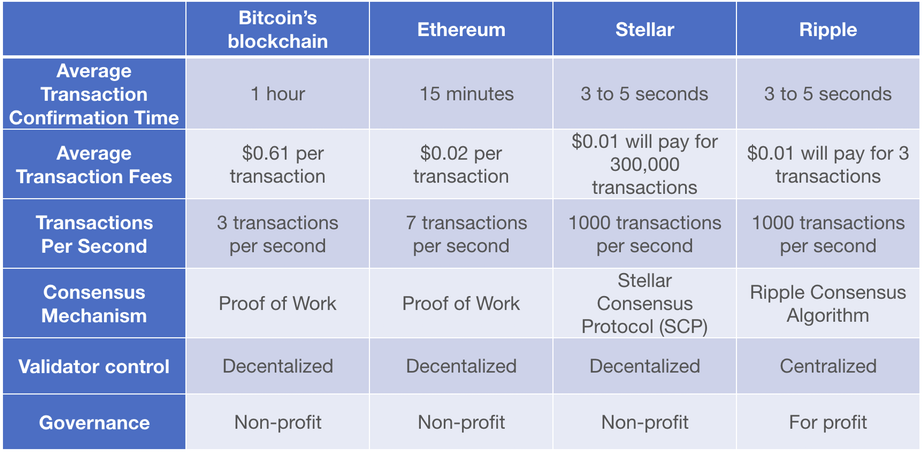
\includegraphics[width=0.90\textwidth]{tps_speed2.png}
  \caption{Comparison of transactions per second of the major blockchains today.}
    \label{fig:tps_speed}
\end{figure}

\subsection{Performance considerations}
When thinking of performance, one of the key metrics that is hotly debated in the community is transactions per second.
Bitcoin is know for its long time to produce a block, on the order of minutes which limits the number of transactions
the network can process. Figure \ref{fig:tps_speed} shows a comparison of the major blockchains today with respect to
this crucial metric. Note that these blockchains shown in the Figure are primarily evaluated against the concept of a
transaction which represents a transfer of assets, goods or monetary value digitally on the blockchain. Stellar and
Ripple are two blockchains that have gained popularity for financial transactions as they tout a higher transaction
velocity. 

In the context of Latitude, the performance of the blockchain is important. The blockchain will handle different types
of data and transactions which will require different levels of consensus and trust. Figure \ref{fig:tps_lat} shows the
different types of transactions that the Latitude blockchain can process and the performance we expect to achieve. Shown
are four types of transactions:
\begin{itemize}
    \item Datastore transactions: These refer to basic transactions to store data values into the geo-spatial data
        store. For instance, if a user shares their driving data, this can include the sensor information, lat/lng of
        the trip taken and any mapping data collected. For ride-sharing applications, this can include any multi-model
        ride details that the user has booked. We expect the blockchain to be able to process close to 1-10 million
        transactions per second, since most such transactions require very low level of consensus and can tolerate 
        eventual consistency \cite{eventual_con}.
    \item Algorithmic computations: These refer to transactions which include executing known algorithms on the
        blockchain. For instance, this could include the computation of various driver behavior algorithms with the
        computation being shared among certain participants on the network. Another computation could include statistics
        such as real-time traffic or aggregate traffic statistics shared with a city for better zoning and planning
        purposes. The amount of consensus required is relatively small but higher than datastore operations in order to
        ensure correct execution of algorithms and lack of malicious intent. Also such operations would require strong
        consistency for their CRUD functionalities. We expect the Latitude design to support 10-100K transactions per
        second at its peak usage.
    \item Data sharing contracts: These transactions refer to the creation, deletion or arbitration of long-term sharing
        smart contracts between participating entities. For instance, it could include a new contract between an
        insurance company and a data provider for sharing certain types of driver score data for certain geographic
        locations. Since these transactions have higher value they require larger amount of trust and consensus in the
        system. Latitude shall support a transaction speed of around 100-1000 transactions per second for this category.
    \item Governance operations: The Governance operations require the highest amount of trust and full consensus of the
        network. These include voting to add/remove council members, critical council decisions such as forks or
        updates/upgrades, decisions on high-value smart contract disputes, etc. The transaction velocity is low for
        reasons of trust, accuracy and correctness and thus we expect the Latitude blockchain to support 1-10
        transactions per second under this category.

\end{itemize}

Another metric of importance for Latitude is the storage capacity in the network. This can be important for
datastore operations. We expect the storage capacity, network bandwidth and any other computing resource to become
available on an incentivized model as determined by usage contracts. For instance, if a user is willing to share data with
a data consumer, the consumer should be able to allocate token resources to provision the network with sufficient
storage. The token can be used to purchase storage using other blockchain storage providers such as Filecoin, Siacoin or
Golem can be used to incentivized nodes to directly supplant on-chain storage.

\begin{figure}[t]
    \centering
    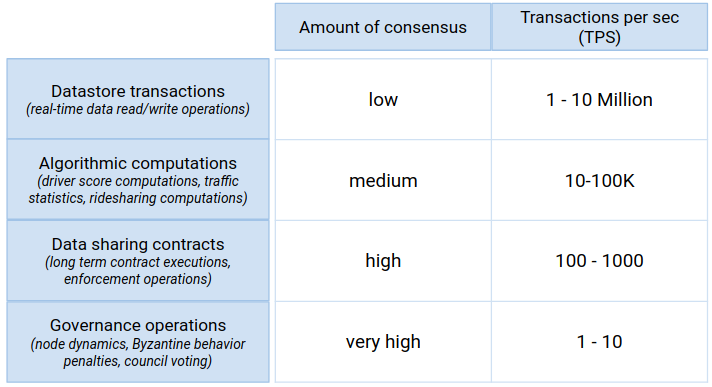
\includegraphics[width=0.75\textwidth]{tps_lat2.png}
  \caption{Expected Transaction per second velocity of various types of functionalities on the Latitude Blockchain.}
    \label{fig:tps_lat}
\end{figure}

